\documentclass[12pt]{article}

\usepackage[utf8]{inputenc}
\usepackage[greek,english]{babel}
\usepackage[unicode]{hyperref}
\usepackage{alphabeta}
\usepackage{amsmath}
\usepackage{mathtools}
\newcommand{\Lagr}{\mathcal{L}}
\usepackage{graphicx}
\usepackage{bookmark}
\usepackage{amsfonts}
 
\begin{document}

\author{Κωνσταντίνος Λέτρος 8851}

 \begin{titlepage} % Suppresses displaying the page number on the title page and the subsequent page counts as page 1
	\newcommand{\HRule}{\rule{\linewidth}{0.5mm}} % Defines a new command for horizontal lines, change thickness here
	
	\center % Centre everything on the page
	
	%------------------------------------------------
	%	Headings
	%------------------------------------------------
	
	\textsc{\LARGE ΠΟΛΥΤΕΧΝΙΚΗ ΣΧΟΛΗ ΑΠΘ}\\[1.5cm] % Main heading such as the name of your university/college
	
	\textsc{\Large ΤΜΗΜΑ ΗΛΕΚΤΡΟΛΟΓΩΝ ΜΗΧΑΝΙΚΩΝ ΚΑΙ ΜΗΧΑΝΙΚΩΝ ΥΠΟΛΟΓΙΣΤΩΝ}\\[0.5cm] % Major heading such as course name
	
	 
	
	%------------------------------------------------
	%	Title
	%------------------------------------------------
	
	\HRule\\[0.4cm]
	
	{\huge\bfseriesΠροσομοίωση και Μοντελοποίηση Συστημάτων}\\[0.4cm] % Title of your document
	
	\HRule\\[1.5cm]
	
	%------------------------------------------------
	%	Author(s)
	%------------------------------------------------
	{\huge\bfseries Κωνσταντίνος Λέτρος \newline 8851}\\[0.4cm]	
	\vfill	
	{\huge\bfseries Εργασία 3}\\[0.4cm]  % Title of your document
	% If you don't want a supervisor, uncomment the two lines below and comment the code above
	%{\large\textit{Author}}\\
	%John \textsc{Smith} % Your name
	
	%------------------------------------------------
	%	Date
	%------------------------------------------------
	
	\vfill\vfill\vfill % Position the date 3/4 down the remaining page
	
	{\large\today} % Date, change the \today to a set date if you want to be precise
	
	%------------------------------------------------
	%	Logo
	%------------------------------------------------
	
	%\vfill\vfill
	%\includegraphics[width=0.2\textwidth]{placeholder.jpg}\\[1cm] % Include a department/university logo - this will require the graphicx package
	 
	%----------------------------------------------------------------------------------------
	
	\vfill % Push the date up 1/4 of the remaining page
	
\end{titlepage}





\newpage
\section{Μέθοδος Κλίσης με Προβολή - Θέμα}
\subsection{Θεωρητική Ανάλυση}
Δίνεται το σύστημα
\[ \dot{x}=ax+bu , \quad x(0)=0 \quad (1.1)\]
για το οποίο θέλουμε να εκτιμήσουμε τις παραμέτρους $a=-1.2 ,\quad b=1.55$.
Γνωρίζουμε ότι για τις παραμέτρους προς εκτίμηση ότι ισχύουν οι παρακάτω περιορισμοί
\[-2<a<0 \]
\[ 1.1 \leq b \leq 2  \]
Η μέθοδος της κλίσης με προβολή μας επιτρέπει να εισάγουμε περιορισμούς στις πιθανές τιμές των εκτιμήσεων των παραμέτρων, όταν αυτοί είναι γνωστοί ή λογικοί λόγω της φυσικής του προβλήματος. Έτσι επιτυγχάνουμε να περιορίσουμε το χώρο αναζήτησης των παραμέτρων μας, από ολόκληρο το $\mathbb{R}^n$ σε ένα υποσύνολό του και να αυξήσουμε την ταχύτητα εύρεσής τους. (όπου n το πλήθος των παραμέτρων προς εκτίμηση).
\\ \\ 
Ως είσοδο $u$ του συστήματος επιλέγουμε την
\[u(t)=5sin(3t)\]
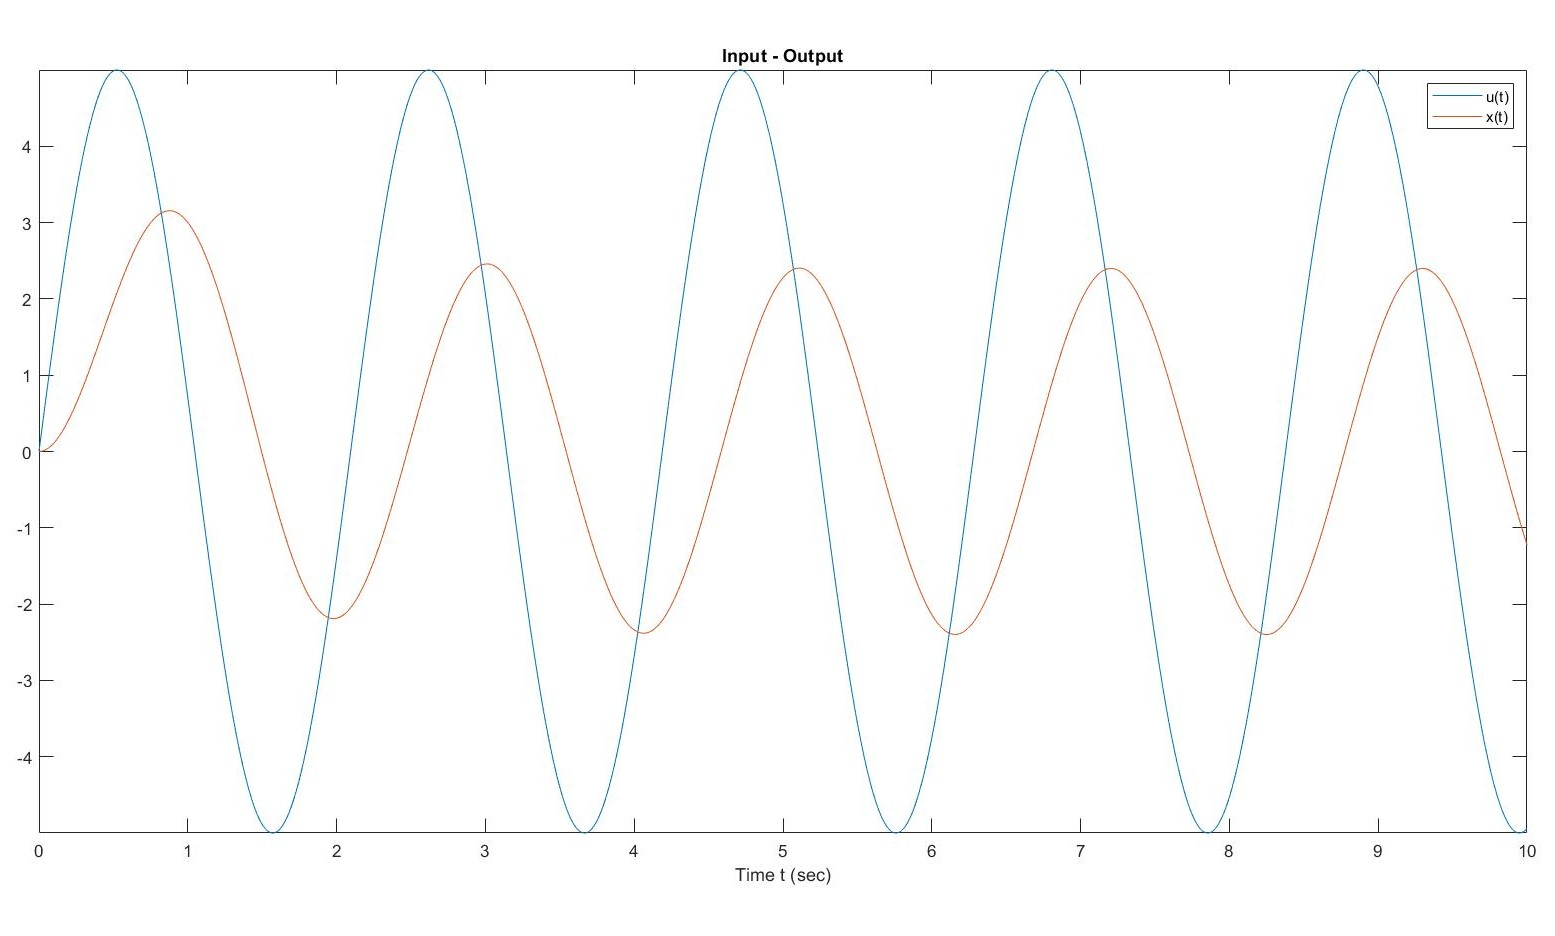
\includegraphics[width=\linewidth]{inpOut.jpg}
\centerline{Σχήμα 1: Είσοδος και Έξοδος του Συστήματος}
\\ \\ \\
Για να εκτιμήσουμε, λοιπόν, τις ζητούμενες παραμέτρους με τη μέθοδο της κλίσης με Προβολή, γραμμικοποιούμε παραμετρικά το σύστημα ως εξής
\[ \dot{x}=ax+bu \Leftrightarrow \dot{x}=ax+bu+\theta_mx-\theta_mx \Leftrightarrow\]
\[\dot{x}+\theta_mx=(\theta_m+a)x+bu \xRightarrow{\Lagr(\cdot)} \]
\[ (s+\theta_m)X(s)=(\theta_m+a)X(s)+bU(s) \Rightarrow\]
\[ X(s)=(\theta_m+a)\cdot \frac{ X(s)}{s+\theta_m} +b \cdot \frac{U(s)}{s+\theta_m} \Rightarrow \]
\[X(s)=\hat{\theta}^{T}\phi \]
όπου
\[
\hat{\theta}=\left[ \hat{\theta_{1}} \quad \hat{\theta_{2}} \right]^{T}=[\theta_m+\hat{a} \quad \hat{b}]^{T} \qquad \text{και} \qquad \phi=\left[ \phi_{1} \quad \phi_{2} \right]^{T}=\left[\frac{ X(s)}{s+\theta_m} \quad \frac{ U(s)}{s+\theta_m}\right]^{T} \]
\\ \\
Από τους περιορισμούς για τις εκτιμήσεις των παραμέτρων προκύπτουν τα εξής: 
\[ -2<\hat{a} \Rightarrow -\hat{a}-2<0 \Rightarrow -\hat{a}-\theta_m+\theta_m-2<0 \Rightarrow -\hat{\theta_1}+\theta_m-2<0 \]
\[ \hat{a}<0 \Rightarrow \hat{a}+\theta_m-\theta_m <0 \Rightarrow \hat{\theta_1}-\theta_m<0 \]
\[ 1.1 \leq \hat{b} \Rightarrow 1.1-\hat{b} \leq 0 \Rightarrow -\hat{\theta_2}+1.1 \leq 0 \]
\[ \hat{b} \leq 2 \Rightarrow \hat{b}-2 \leq 0 \Rightarrow \hat{\theta_2}-2 \leq 0 \]
Λόγω των παραπάνω σχέσεων θεωρούμε τα εξής
\[ g_1(\hat{\theta_1})=-\hat{\theta_1}+\theta_m-2\]
\[ g_2(\hat{\theta_1})=\hat{\theta_1}-\theta_m\]
\[ g_3(\hat{\theta_2})=-\hat{\theta_2}+1.1\]
\[ g_4(\hat{\theta_2})=\hat{\theta_2}-2\]
 με \[ \nabla_{\hat{\theta}} g_1 = 
 \begin{bmatrix}
-1  \\ 
 0
\end{bmatrix}
\quad 
\nabla_{\hat{\theta}} g_2 = 
 \begin{bmatrix}
1 \\ 
0
\end{bmatrix}
\quad
\nabla_{\hat{\theta}} g_3 = 
 \begin{bmatrix}
0  \\ 
-1
\end{bmatrix}
\quad 
\nabla_{\hat{\theta}} g_4 = 
 \begin{bmatrix}
0 \\ 
1
\end{bmatrix}
\quad
\]
όπου η συναρτήσεις $g$ εκφράζουν τα σύνορα ενός κυρτού συνόλου Θ, εντός του οποίου επιθυμούμε να παραμείνει η τροχιά του $\hat{\theta}$ και το οποίο είναι το εξής:
\[ \Theta= \left \{ \hat{\theta} \in \mathbb{R}^2 : g(\hat{\theta}) \leq 0 \right \} \] 
Από τον πίνακα $\phi$ έχουμε
\[ (s+\theta_m)\phi_1=X(s) \xRightarrow{\Lagr^{-1}(\cdot)} \frac{d\phi_{1}}{dt}+\theta_m\phi_{1}=x \quad (1.2)\]
\[ (s+\theta_m)\phi_2=U(s) \xRightarrow{\Lagr^{-1}(\cdot)} \frac{d\phi_{2}}{dt}+\theta_m\phi_{2}=u \quad (1.3)\]
\\
Στη συνέχεια ορίζουμε τη συνάρτηση σφάλματος $e$, ως εξής
\[ e=x-\hat{x}=x-\hat{\theta}^{T}\phi = (\theta^{*}-\hat{\theta})^{T} \phi \]
και μια συνάρτηση κέρδους, $K(\theta)$, η οποία είναι κυρτή ώστε να παρουσιάζει μοναδικό ολικό ελάχιστο (ή όλα τα τοπικά ελάχιστα συμπίπτουν με το ολικό) που ελαχιστοποιεί το σφάλμα.
\[ K(\hat{\theta})=\frac{1}{2}ee^{T} \Rightarrow\]
\[ K(\hat{\theta})=\frac{1}{2}(x-\hat{\theta}^{T}\phi)(x^{T}-\phi^{T}\hat{\theta}) \Rightarrow\]
\[ K(\hat{\theta})=\frac{1}{2}(xx^{T}-x\phi^{T}\hat{\theta} - \hat{\theta}^{T}\phi x+\hat{\theta}^{T}\phi\phi^{T}\hat{\theta}) \]
Σύμφωνα με τη μέθοδο της κλίσης, για κάποιο διαγώνιο και θετικά ορισμένο πίνακα $\Gamma$ τον οποίο επιλέγουμε εμείς ώστε να επιτύχουμε μεγαλύτερη ταχύτητα σύγκλισης και ομαλή απόκριση της εκτίμησης του $\hat{\theta}$ στην πραγματική του τιμή, θέτουμε
\[ \dot{\hat{\theta}}=Proj \{ -\Gamma \nabla_{\hat{\theta}} K(\hat{\theta}) \} \]
όπου $Proj \{ -\Gamma \nabla_{\hat{\theta}} K(\hat{\theta}) \}=$
$ \left\{
    \begin{array}{l}
        -\Gamma \nabla K , \quad \hat{\theta} \in \Theta_{in}\cup \{ \partial\Theta \cap [ -(\Gamma \nabla_{\hat{\theta}} K)^{T} \cdot \nabla g \leq 0 ] \} \\
        -\Gamma \nabla K + \Gamma \frac{\nabla g \nabla    g^{T}}{\nabla g^{T} \Gamma \nabla g}\Gamma \nabla K, \quad \text{διαφορετικά} \\   
    \end{array}
    \right.$
\\ \\ \\
Επομένως όταν οι εκτιμήσεις $\hat{\theta}$ ανήκουν στο εσωτερικό του $\Theta$ ή στο σύνορο $\partial \Theta$ με κατεύθυνση προς το εσωτερικό του, έχουμε
\[\dot{\hat{\theta}}=-\frac{\Gamma}{2}(-2\phi x^{T} +2\phi\phi^{T}\hat{\theta})\Rightarrow\] 
\[\dot{\hat{\theta}}= \Gamma(\phi x^{T} -\phi\phi^{T}\hat{\theta})  \Rightarrow \]
\[\dot{\hat{\theta}} =\Gamma \phi e^{T} \Rightarrow\]
\[ 
\begin{bmatrix}
 \dot{\hat{\theta_1}} \\
  \dot{\hat{\theta_2}} 
\end{bmatrix}= 
\begin{bmatrix}
    \gamma_1 & 0 \\
    0 & \gamma_2
\end{bmatrix}
 \begin{bmatrix}
  \phi_{1} \\
   \phi_{2} \end{bmatrix}
 x -
 \begin{bmatrix}
    \gamma_1 & 0 \\
    0 & \gamma_2
\end{bmatrix}
 \begin{bmatrix}
  \phi_{1} \\
   \phi_{2} 
\end{bmatrix} 
 \left[ \phi_{1} \quad \phi_{2} \right]
 \begin{bmatrix}
  \hat{\theta_1} \\
 \hat{\theta_2} 
 \end{bmatrix}  \]
\\
Από όπου προκύπτουν τελικά οι γραμμικές διαφορικές εξισώσεις
\\ \\
$
\left\{
\begin{array}{ll}
\dot{\hat{\theta_1}}=\gamma_1 (\phi_{1}x-\phi_1^{2}\hat{\theta_1}-\phi_{1}\phi_{2}\hat{\theta_{2}})
\\
\dot{\hat{\theta_2}}=\gamma_2 (\phi_{2}x-\phi_{2}\phi_{1}\hat{\theta_1}-\phi_2^{2}\hat{\theta_{2}}) 
\end{array}
\right.
$
\\ \\ \\
Διαφορετικά έχουμε
\[\dot{\hat{\theta}}=\left( I - \Gamma \frac{\nabla g \nabla    g^{T}}{\nabla g^{T} \Gamma \nabla g}\right) (-\Gamma \nabla K)  \]
όπου η επιλογή του $g$ εξαρτάται από την κατεύθυνση του $\hat{\theta}$. Αν, για παράδειγμα, το $\hat{\theta_1}$ πλησιάζει την οριακή τιμή $\theta_m-2$ με κατεύθυνση προς το εξωτερικό του Θ, τότε για τον υπολογισμό του παραπάνω όρου χρησιμοποιείται η $g_1$. Έτσι ο όρος $\Gamma \frac{\nabla g \nabla    g^{T}}{\nabla g^{T} \Gamma \nabla g }\Gamma \nabla K$ θα αναγκάσει το $\hat{\theta_1}$ να παραμείνει στο σύνορο $\partial \Theta$ μέχρι τελικά να επιστρέψει εντός του Θ. Όμοια για τα υπόλοιπα τρία όρια-περιορισμούς χρησιμοποιούνται οι αντίστοιχες $g$.
\\ \\
Έτσι προκύπτουν άλλες δύο διαφορικές εξισώσεις για ως προς $\hat{\theta_1},\hat{\theta_2}$.
\\ \\
Έπειτα, επιλύουμε το σύστημα των πέντε διαφορικών εξισώσεων $(1.1),(1.2),(1.3)$ και των κλαδικών ως προς $\hat{\theta_1},\hat{\theta_2}$ και βρίσκουμε τις εκτιμήσεις $\hat{\theta_1},\hat{\theta_2}$. Τελικά από τον πίνακα $\hat{\theta}$ προκύπτουν οι εκτιμήσεις $\hat{a},\hat{b}$ ως:
\\
\[\hat{a}=\hat{\theta_1}-\theta_m \qquad \text{και} \qquad \hat{b}=\hat{\theta_2}\]
που συμπίπτουν με τις πραγματικές τιμές των παραμέτρων μετά από κάποιο χρονικό διάστημα. Μεγάλη σημασία για την λειτουργία του αλγορίθμου έχει οι αρχικές συνθήκες των δύο τελευταίων διαφορικών εξισώσεων να έχουν τιμές που ανήκουν εντός του συνόλου $Θ$. Σε αντίθετη περίπτωση είναι πιθανό ο αλγόριθμος να οδηγηθεί σε αστάθεια.
\\ \\
Η επιλογή του πίνακα $\Gamma$, δηλαδή των θετικών σταθερών $\gamma_1 $ και $\gamma_2$, εξαρτάται από την επιθυμητή ταχύτητα σύγκλισης των εκτιμήσεων των παραμέτρων στις πραγματικές τους τιμές, αλλά και από την οικονομική δυνατότητα που υπάρχει. Επίσης, η επιλογή μεγάλων τιμών προκαλεί την εμφάνιση απότομων διαταραχών που μπορούν να δημιουργήσουν προβλήματα στην ομαλή λειτουργία του συστήματος.
\\ \\
Η επίλυση το προβλήματος, ωστόσο, δώθηκε και με τη χρήση ενός δεύτερου αλγορίθμου (Αλγόριθμος 3 από $Appendix$ $E$) όμοιας λογικής με του προηγούμενου.
\\ \\
Για τη λειτουργία του αλγόριθμου αυτού πέραν των προηγουμένων ορίζουμε κι ένα νέο σύνολο 
\[ \Theta_{\text{ε}}= \left \{ \hat{\theta} \in \mathbb{R}^2 : g(\hat{\theta}) \leq \text{ε} ,\text{ε}>0 \right \} \]
το οποίο είναι πιο ευρύ από το $\Theta$ και το εμπεριέχει.
\\ \\
Στη συνέχεια ακολουθείται παρόμοια διαδικασία με την προηγούμενη με τη διαφορά ότι αυτή τη φορά θέτουμε:
\[ \dot{\hat{\theta}}=Proj \{ -\Gamma \nabla_{\hat{\theta}} K(\hat{\theta}) \} \]
όπου
\\
$Proj \{ -\Gamma \nabla_{\hat{\theta}} K(\hat{\theta}) \}=$
$ \left\{
    \begin{array}{l}
        -\Gamma \nabla K , \quad \hat{\theta} \in \Theta \cup \{  -(\Gamma \nabla_{\hat{\theta}} K)^{T} \cdot \nabla g \leq 0 \}  \\
        -\Gamma \nabla K + c(\hat{\theta}) \Gamma \frac{\nabla g \nabla    g^{T}}{\nabla g^{T} \Gamma \nabla g}\Gamma \nabla K, \quad \hat{\theta} \in \{ \Theta_{\text{ε}}-\Theta \} \cap \{  -(\Gamma \nabla_{\hat{\theta}} K)^{T} \cdot \nabla g > 0 \} \\   
    \end{array}
    \right.$
\\ \\ \\
με 
\[c(\hat{\theta})=min \left \{ 1, \frac{g(\hat{\theta})}{\text{ε}} \right \}\]
Η προσθήκη του $c(\hat{\theta})$ προσδίδει μια ομαλότερη αλλαγή κατεύθυνσης του $\hat{\theta}$ όταν αυτό κατευθύνεται μακριά από τα όρια που ορίζει το $\Theta$. Συγκεκριμένα, ορίζουμε μια δεύτερη ζώνη πλάτους ε, $(\Theta_{\text{ε}}-\Theta )$ αμέσως έξω από το σύνορο του $\Theta$, εντός της οποίας το $\dot{\hat{\theta}}$ αρχίζει να μειώνεται σταδιακά. Αν, λοιπόν, δεν προλάβει να γίνει αρνητικό όσο βρίσκεται στη δεύτερη ζώνη, ώστε να επιστρέψει εντός του $\Theta$, όταν φτάσει πάνω στο σύνορο $\partial \Theta_{\text{ε}}$ μηδενίζεται μέχρι να γίνει ξανά αρνητικό και να επιστρέψει εντός του $\Theta$.  
\subsection{Αποτελέσματα - Αξιολόγηση}
Η εργασία αποτελείται από δύο αρχεία $Matlab$, τα $algorithmA.m$ και $algorithmB.m$ που περιέχουν τους αλγορίθμους για τη μέθοδο κλίσης με προβολή όπως αναλύεται στη θεωρία και στο $Appendix$ $E$ αντίστοιχα.
\\ \\
Στο αρχείο $algorithmA.m$ επιλύεται το σύστημα διαφορικών εξισώσεων όπως αναλύθηκε στη Θεωρητική Ανάλυση με χρήση της συνάρτησης του $Matlab$, $ode45$, και των $events$ για μέγιστη ακρίβεια ενώ στη συνέχεια παράγονται τα διαγράμματα με τις χρονικές αποκρίσεις των εκτιμήσεων $\hat{a},\hat{b}$, καθώς επίσης και το διαγράμμα που δείχνει την τροχιά των $\hat{a}$,$\hat{b}$ για διάφορες αρχικές συνθήκες.
\\ \\
Όμοια στο αρχείο $algorithmB.m$ περιέχεται ο κώδικας για τον αλγόριθμο από το $Appendix$ $E$ που περιγράφηκε στο τέλος της Θεωρητικής Ανάλυσης.
\\ \\
Για την εκτέλεση του αλγορίθμου επιλέχθηκαν $\theta_m=2$ , $\gamma_1=20$ , $\gamma_2=30$ , $\text{ε}=0.15$ (για το δεύτερο αλγόριθμο), τιμές που προέκυψαν μετά από δοκιμές και δίνουν ικανοποιητικά αποτελέσματα, όπως ομαλές καμπύλες χωρίς πολλές διαταραχές.
\\ \\
Οι γραφικές παραστάσεις με τις χρονικές αποκρίσεις των εκτιμήσεων $\hat{a},\hat{b}$ καθώς και της τροχιάς των $\hat{a}$,$\hat{b}$ και σφάλματος φαίνονται στα Σχήματα 2 έως 8 για τον πρώτο αλγόριθμο με αρχικές τιμές για τα $(\hat{a},\hat{b})$ οι οποίες βρίσκονται εντός του συνόλου Θ όπως απαιτείται, τις
\\
 $(-1.999,2)$ , $(-0.001,2)$ , $(-1.999,1.1)$ , $(-0.001,1.1)$ , $(-0.5,1.2)$ , $(-0.75,1.6)$ , $(-1.8,1.7)$ , $(-1.3,1.2)$.
\\ \\
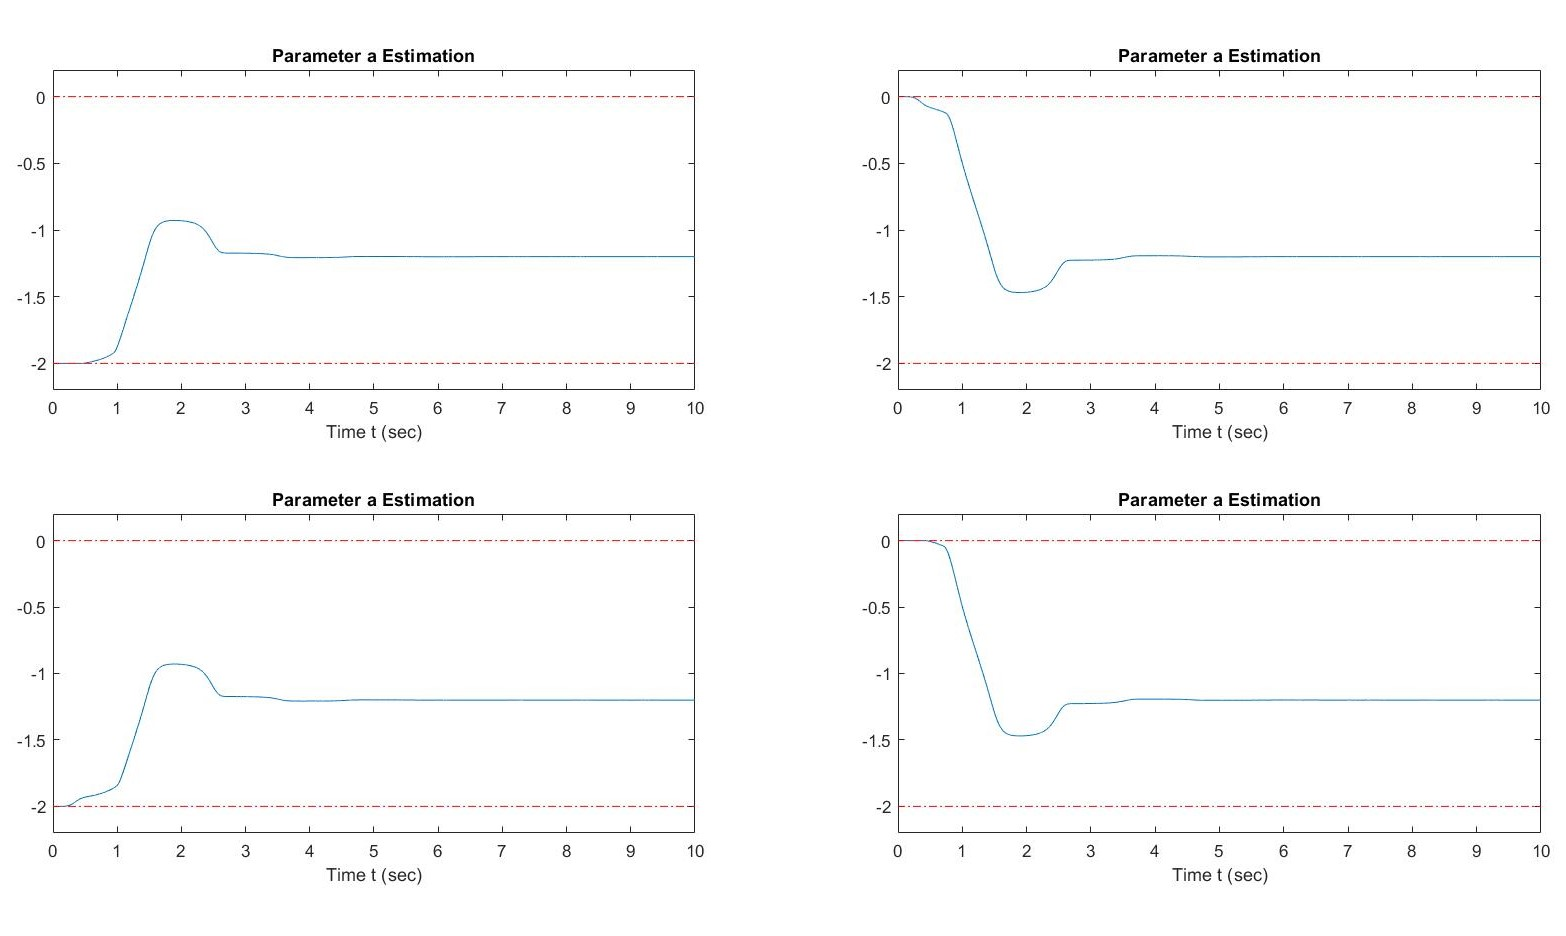
\includegraphics[width=\linewidth]{a_est_a1.jpg}
\centerline{Σχήμα 2: Χρονική Απόκριση Εκτίμησης $\hat{a} \quad (1)$}
\\ \\
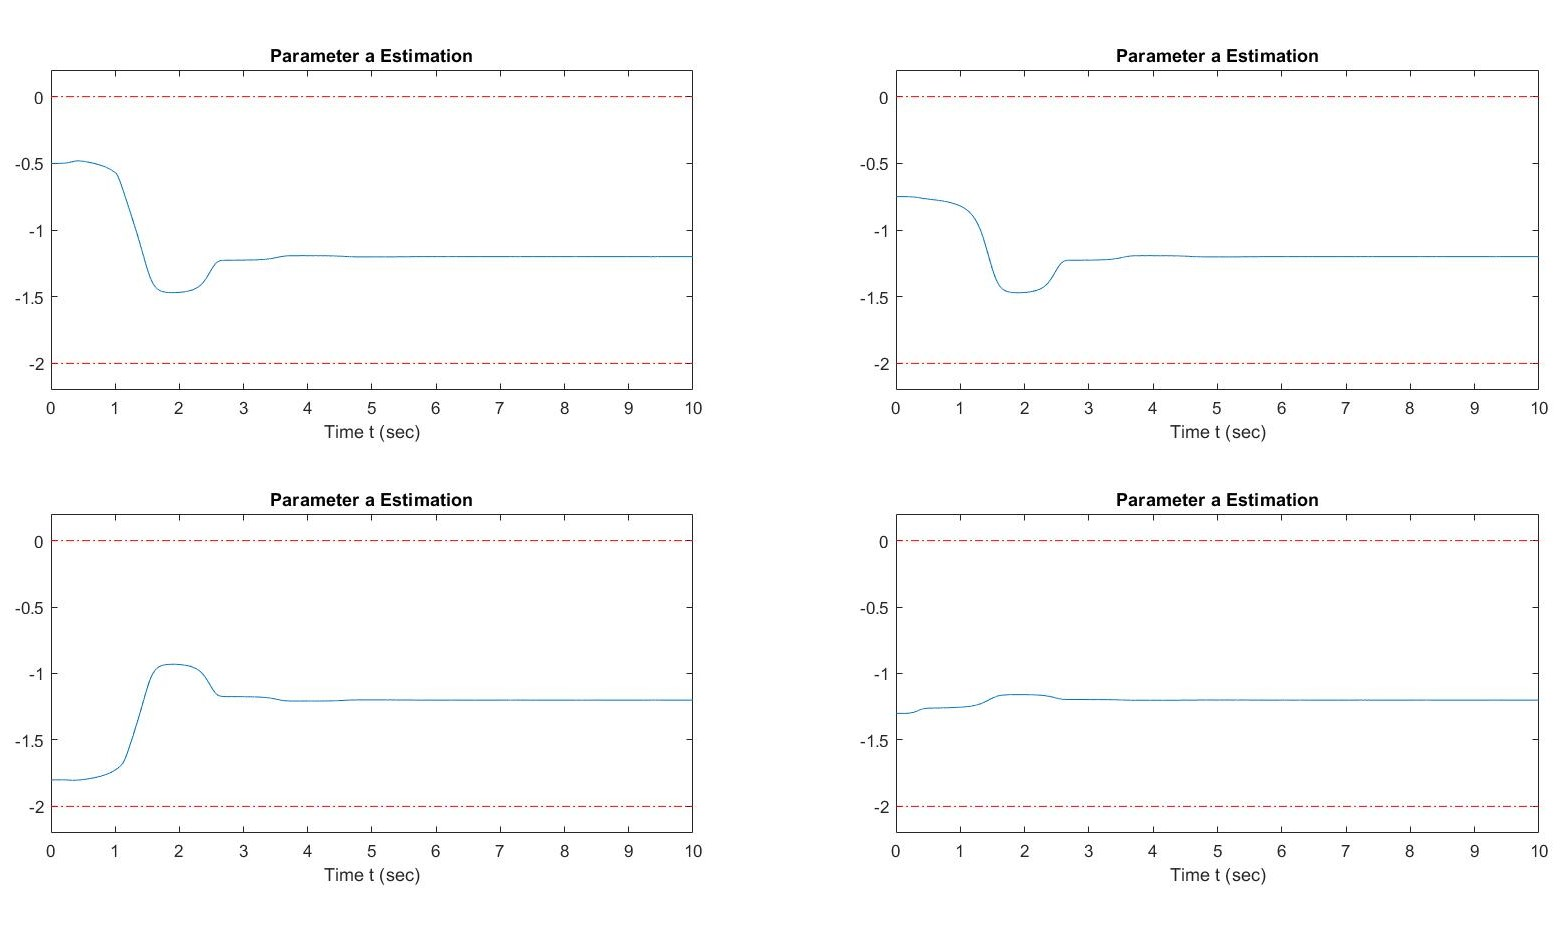
\includegraphics[width=\linewidth]{a_est_a2.jpg}
\centerline{Σχήμα 3: Χρονική Απόκριση Εκτίμησης $\hat{a} \quad (2)$}
\\ \\
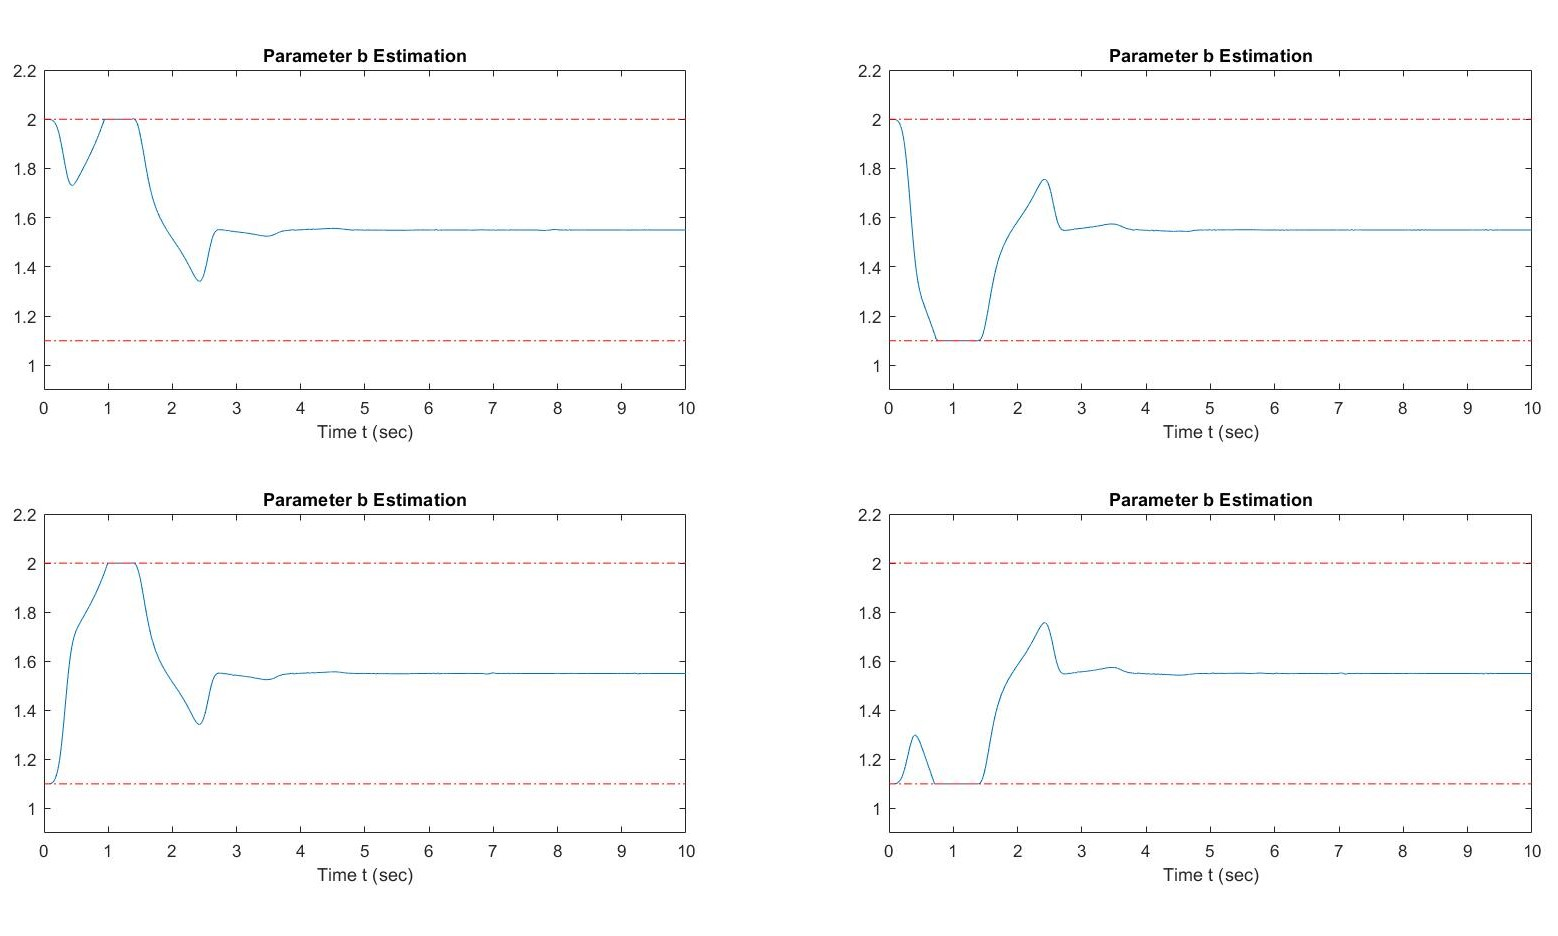
\includegraphics[width=\linewidth]{b_est_a1.jpg}
\centerline{Σχήμα 4: Χρονική Απόκριση Εκτίμησης $\hat{b} \quad (1)$}
\\ \\
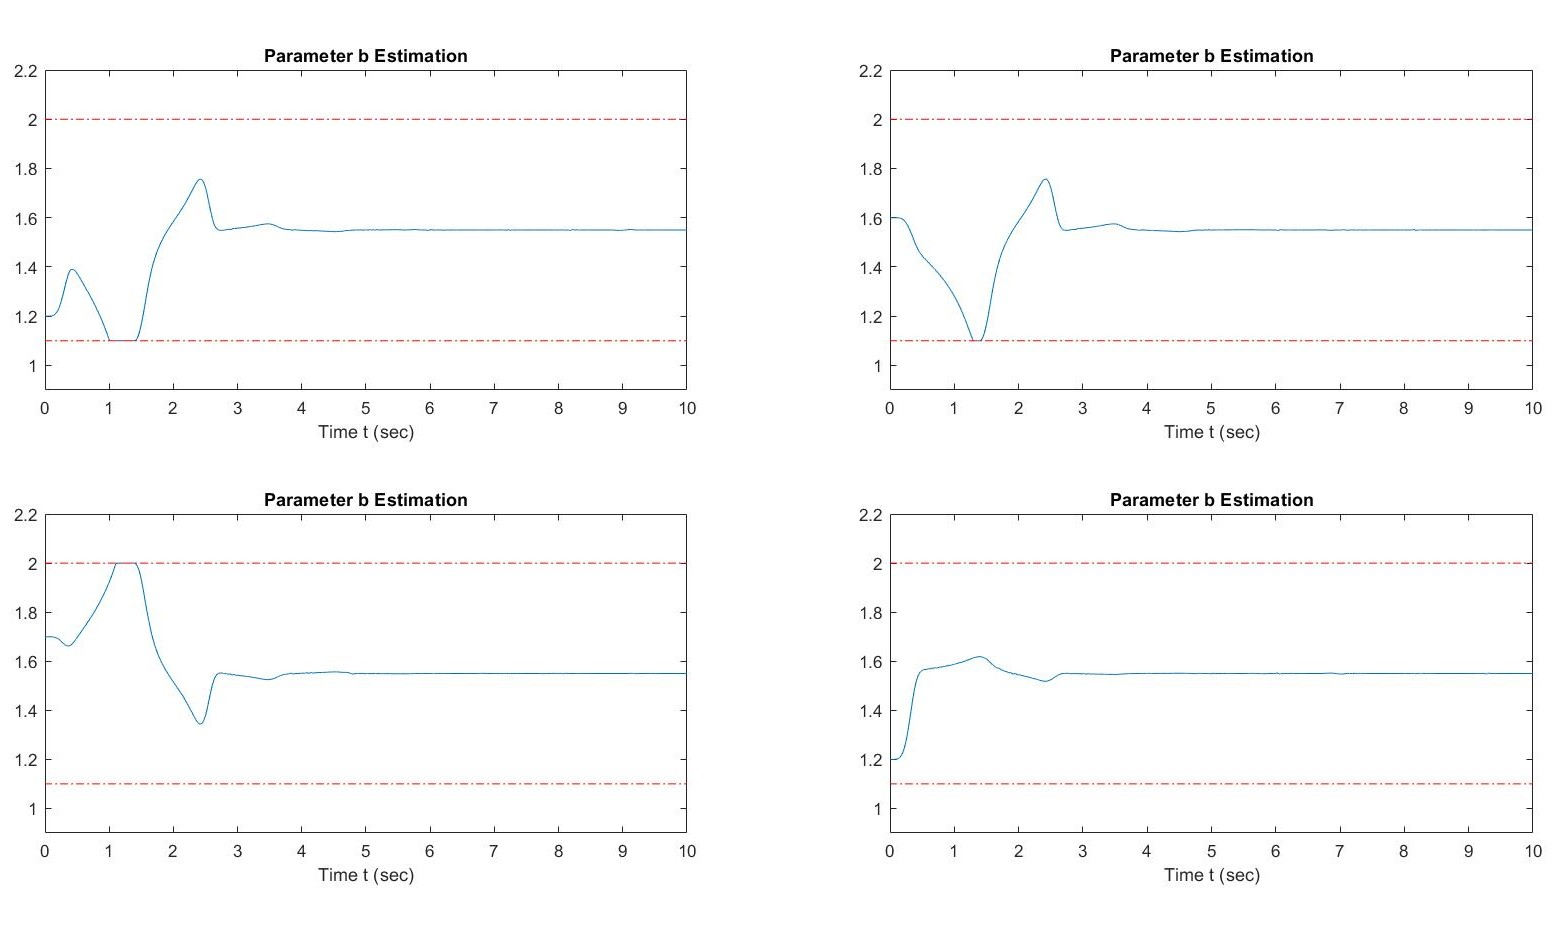
\includegraphics[width=\linewidth]{b_est_a2.jpg}
\centerline{Σχήμα 5: Χρονική Απόκριση Εκτίμησης $\hat{b} \quad (2)$}
\\ \\
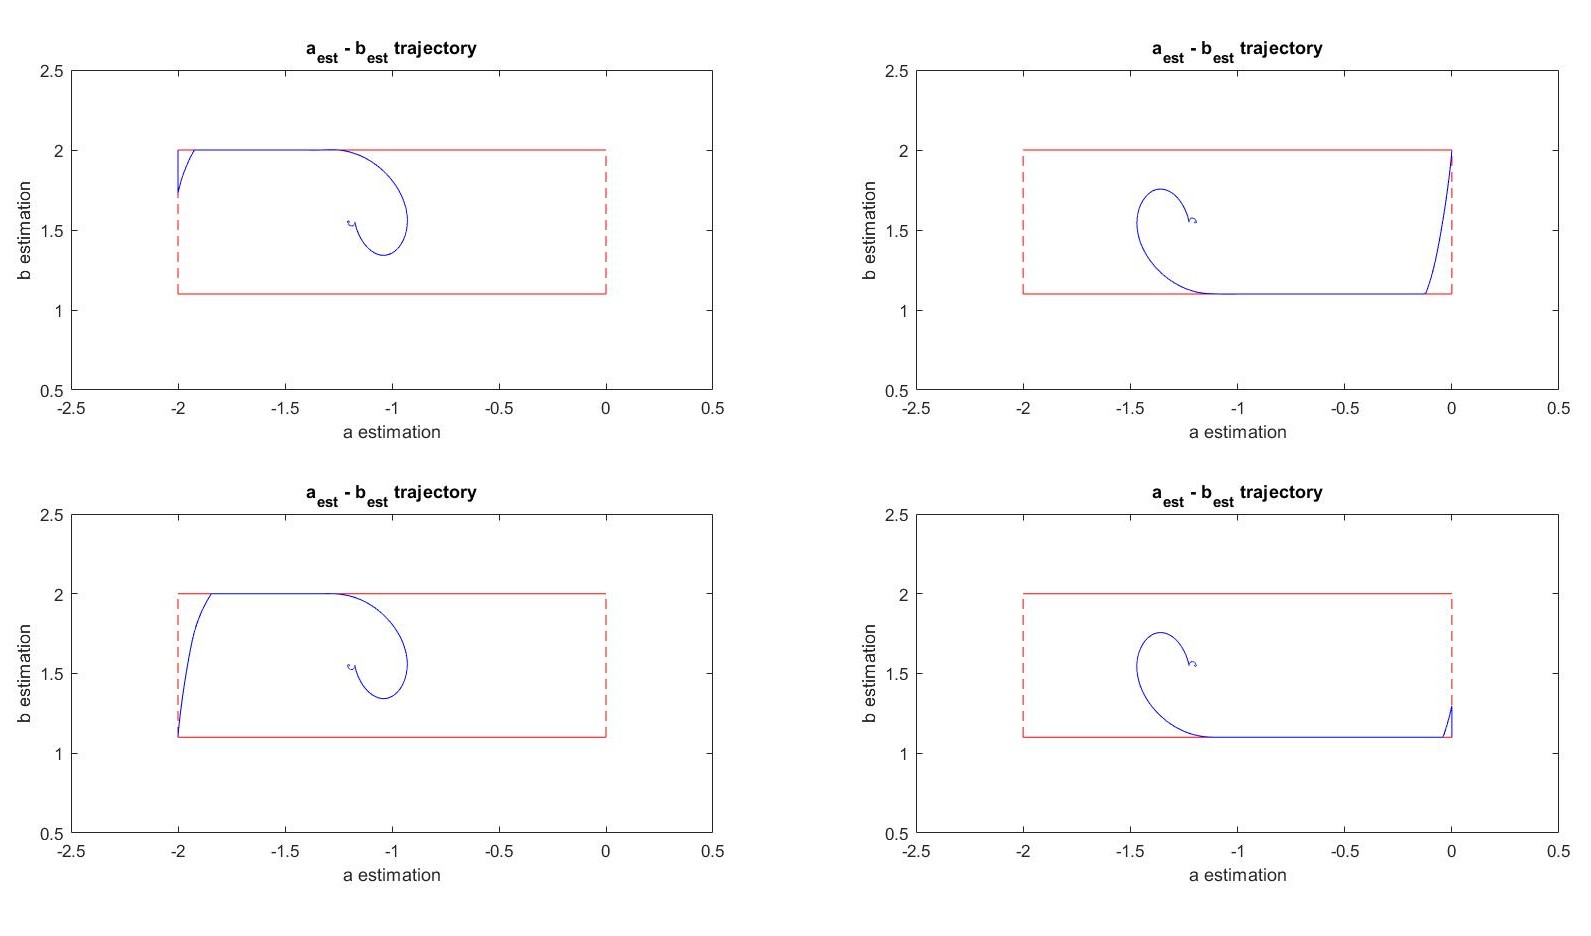
\includegraphics[width=\linewidth]{ab_est_a1.jpg}
\centerline{Σχήμα 6: Τροχιά Εκτιμήσεων στο Επίπεδο $\hat{a} - \hat{b} \quad (1)$}
\\ \\
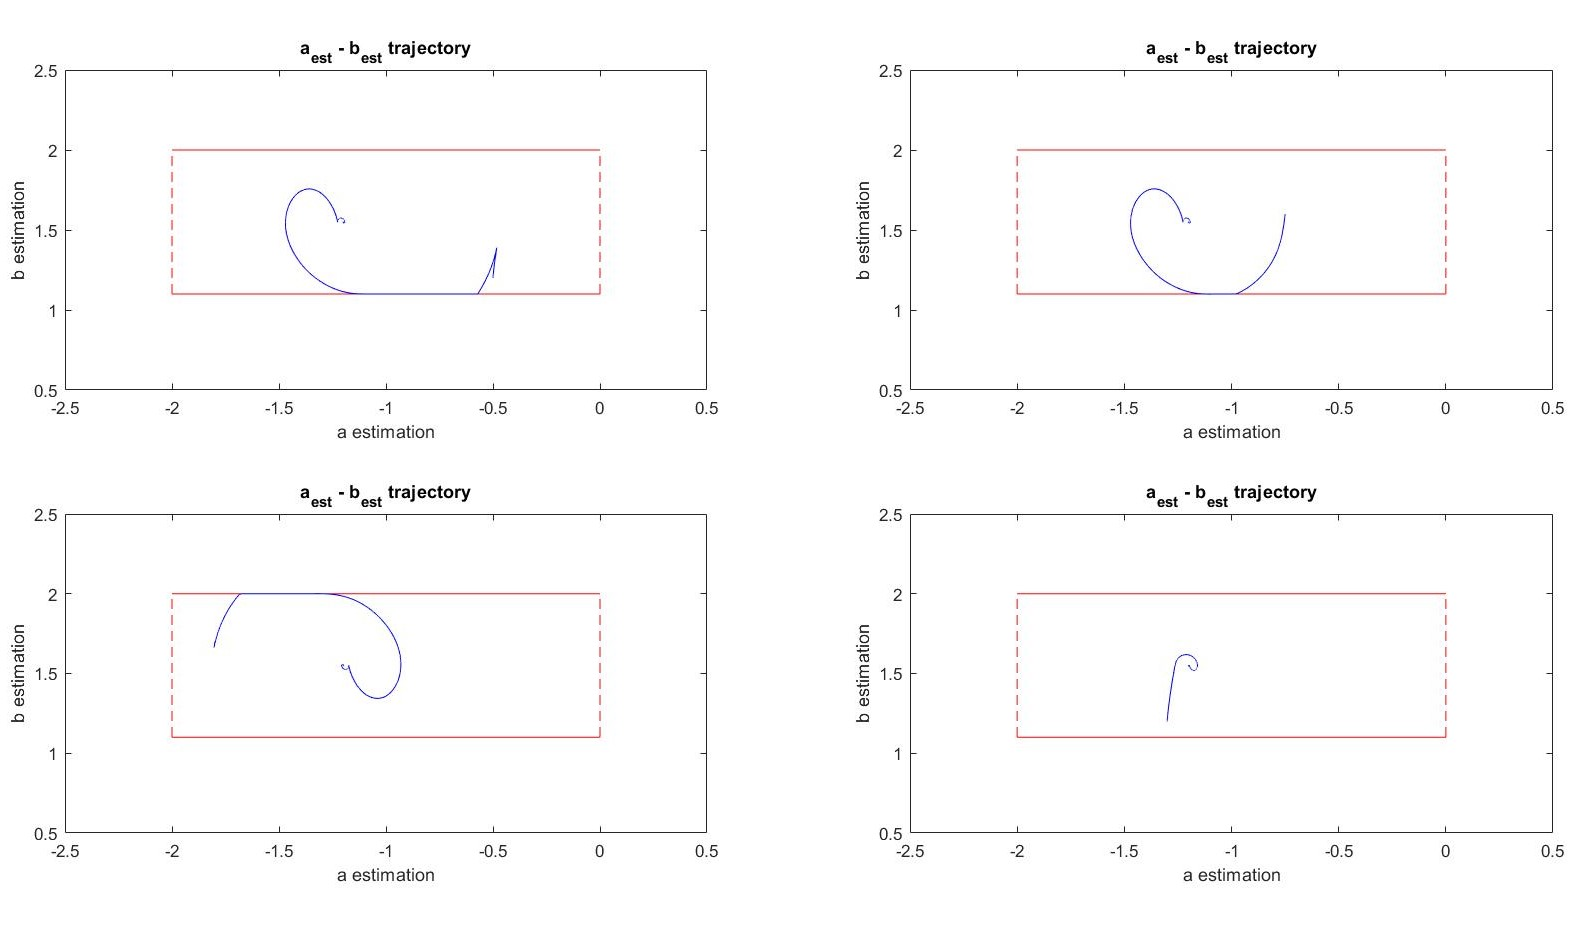
\includegraphics[width=\linewidth]{ab_est_a2.jpg}
\centerline{Σχήμα 7: Τροχιά Εκτιμήσεων στο Επίπεδο $\hat{a} - \hat{b} \quad (2)$}
\\ \\
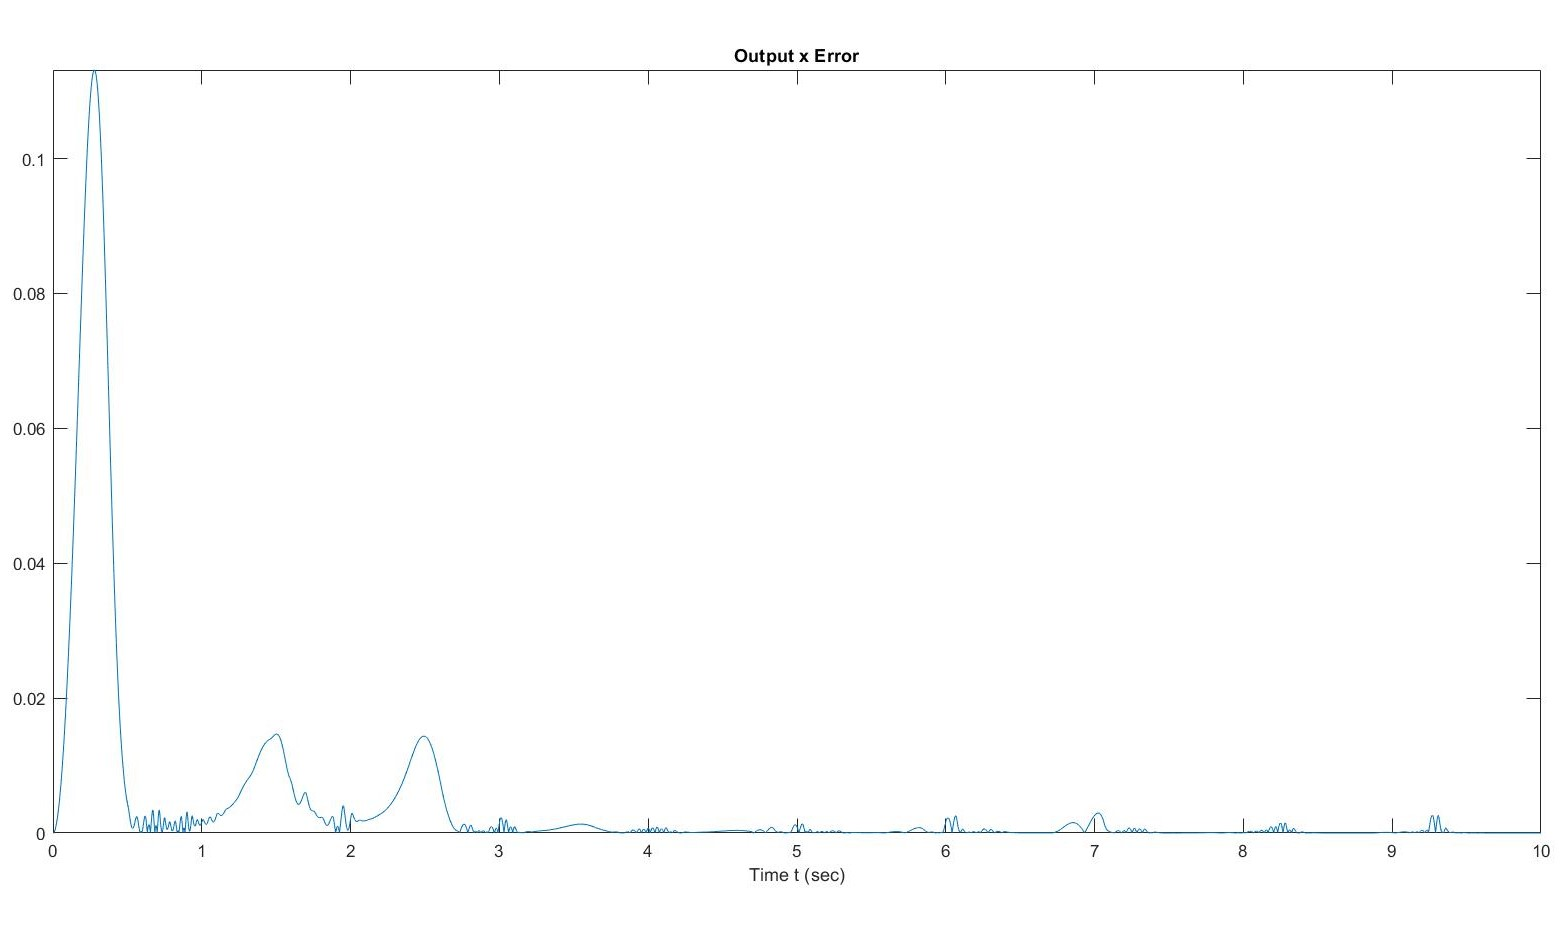
\includegraphics[width=\linewidth]{errorA.jpg}
\centerline{Σχήμα 8: Χρονική Απόκριση Σφάλματος}
\\ \\
Όπως βλέπουμε το σφάλμα για τις αρχικές τιμές $(-1.999,2)$ μετά από λίγο χρόνο είναι αρκετά μικρό, και τελικά σχεδόν μηδενικό, όμως εμφανίζονται μικρές διαταραχές. Όμοια είναι η μορφή του σφάλματος και για τις υπόλοιπες αρχικές τιμές.
\\ \\
Οι αντίστοιχες γραφικές παραστάσεις από το δεύτερο αλγόριθμο, για τις ίδιες αρχικές τιμές, φαίνονται στα Σχήματα 9 έως 15.
\\ \\
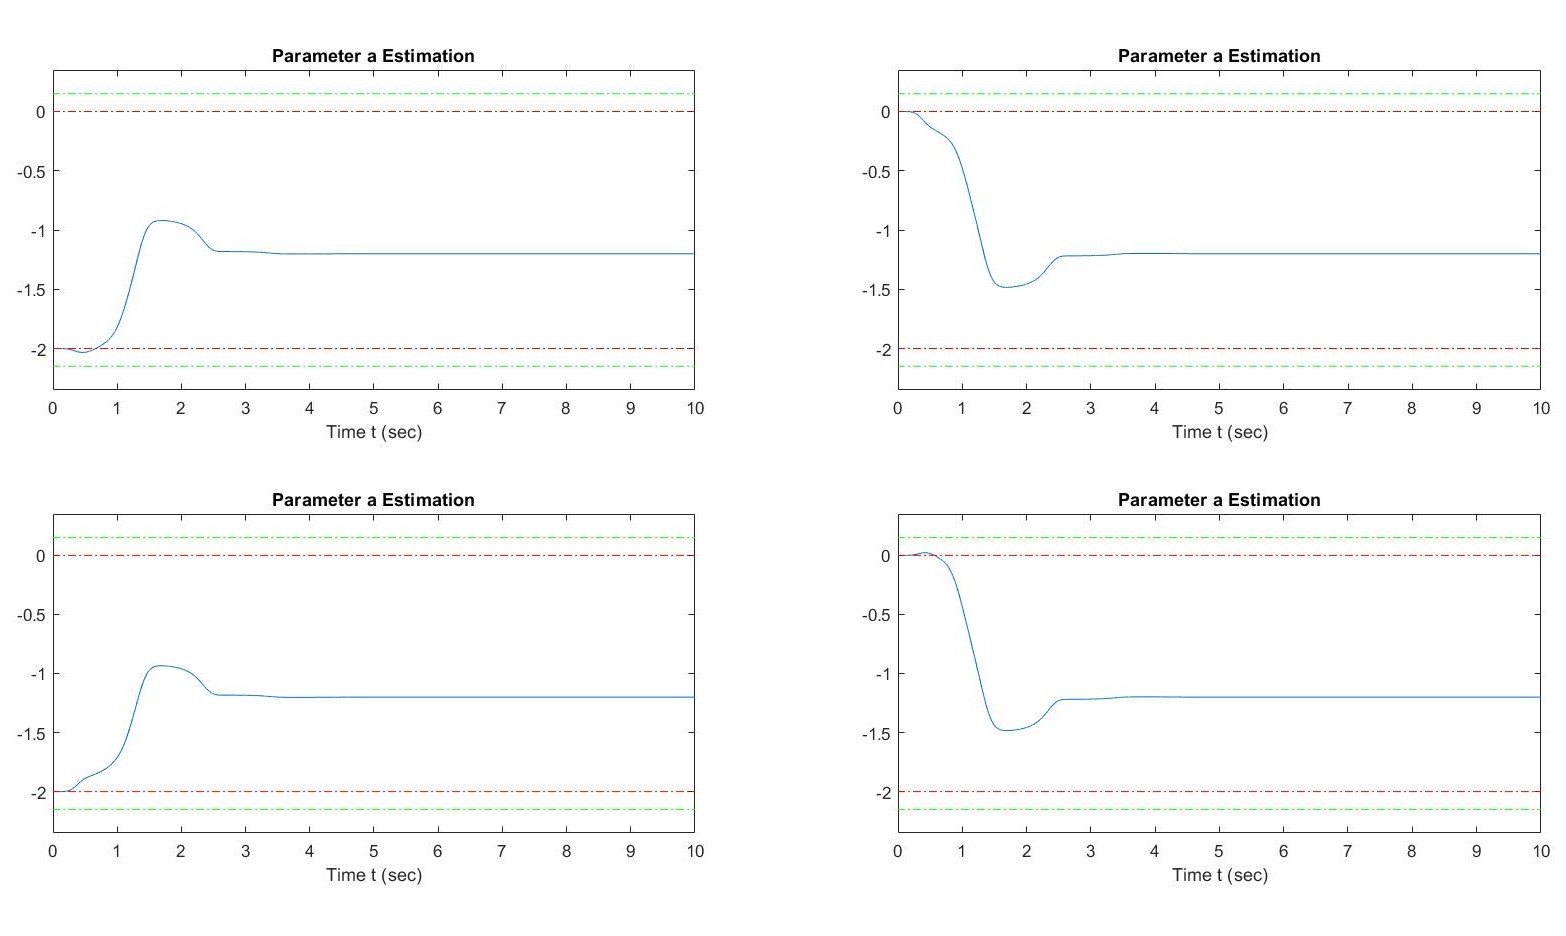
\includegraphics[width=\linewidth]{a_est_b1.jpg}
\centerline{Σχήμα 9:  Χρονική Απόκριση Εκτίμησης $\hat{a} \quad (1)$}
\\ \\
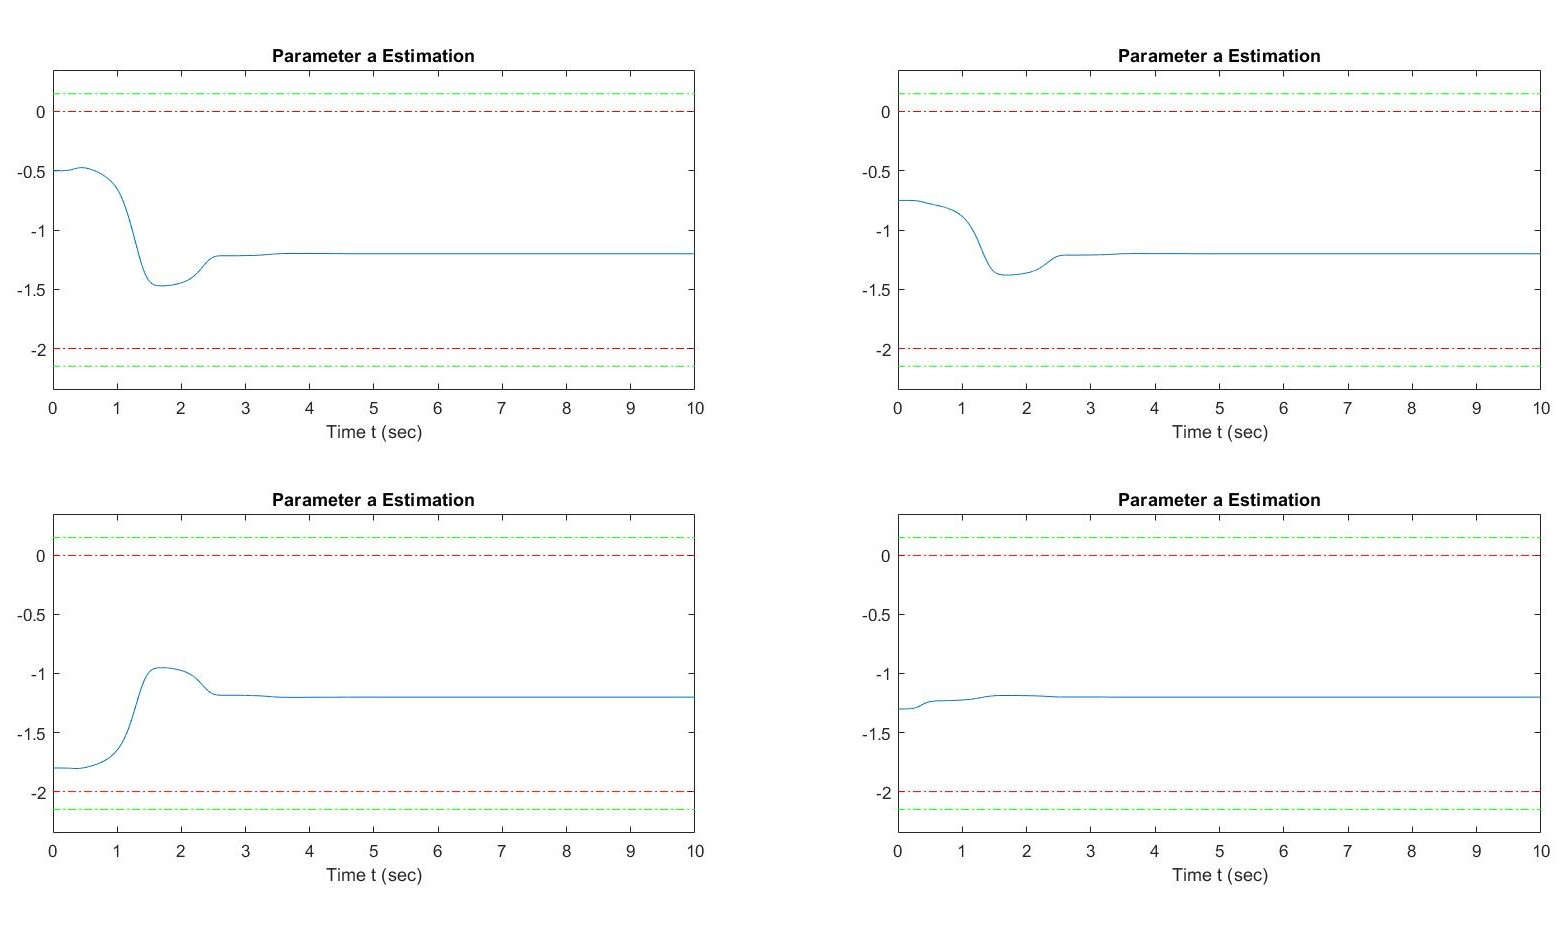
\includegraphics[width=\linewidth]{a_est_b2.jpg}
\centerline{Σχήμα 10:  Χρονική Απόκριση Εκτίμησης $\hat{a} \quad (2)$}
\\ \\
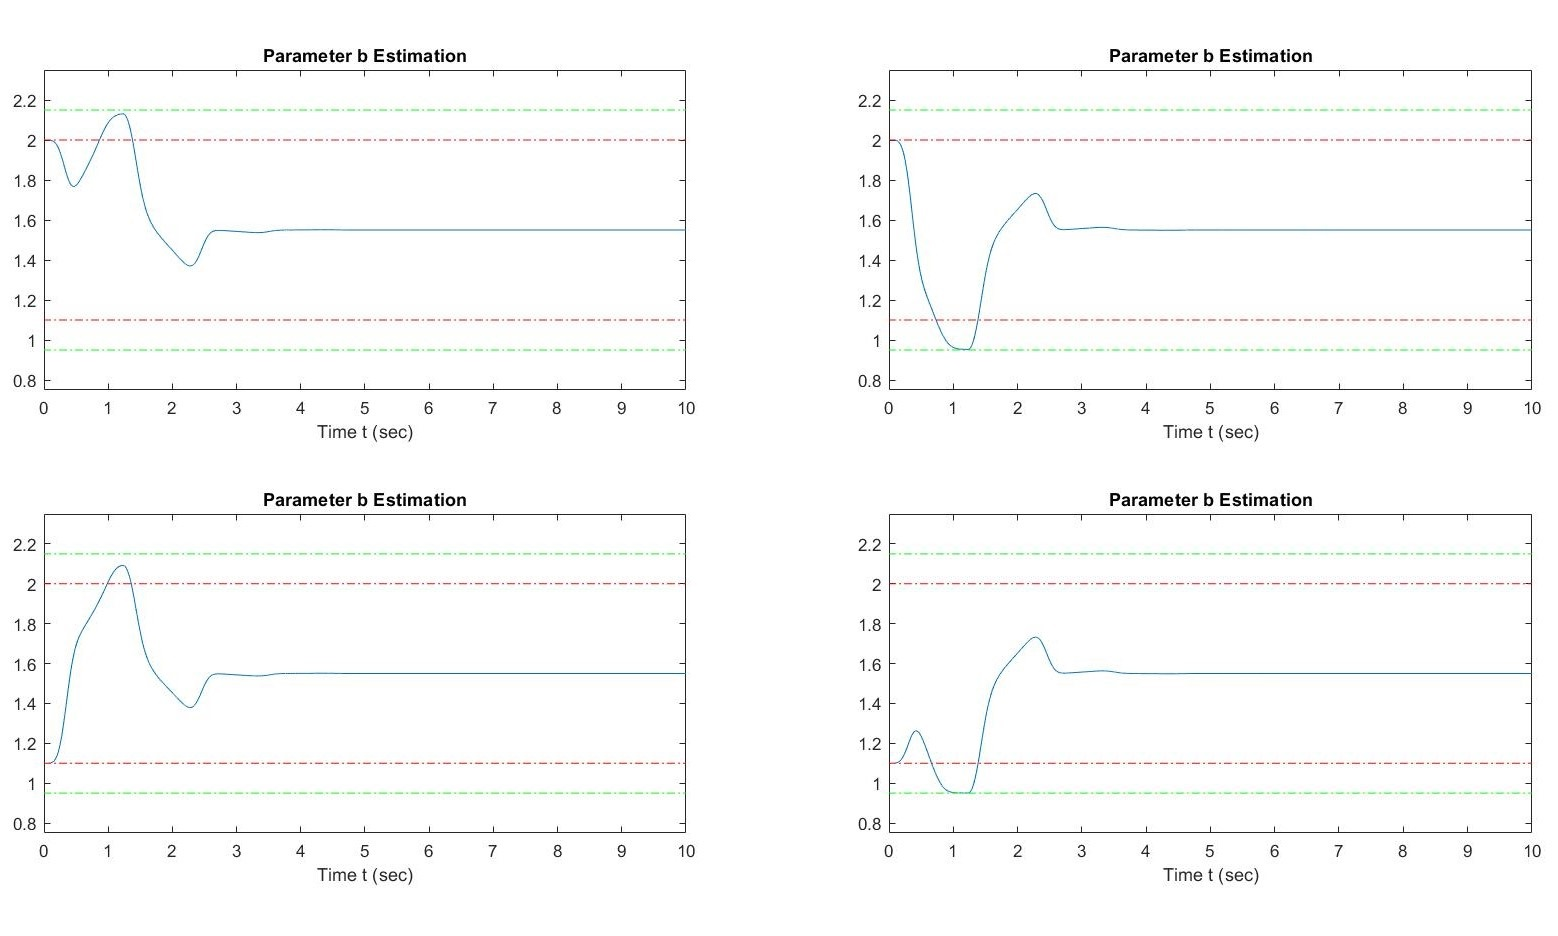
\includegraphics[width=\linewidth]{b_est_b1.jpg}
\centerline{Σχήμα 11:  Χρονική Απόκριση Εκτίμησης $\hat{b} \quad (1)$}
\\ \\
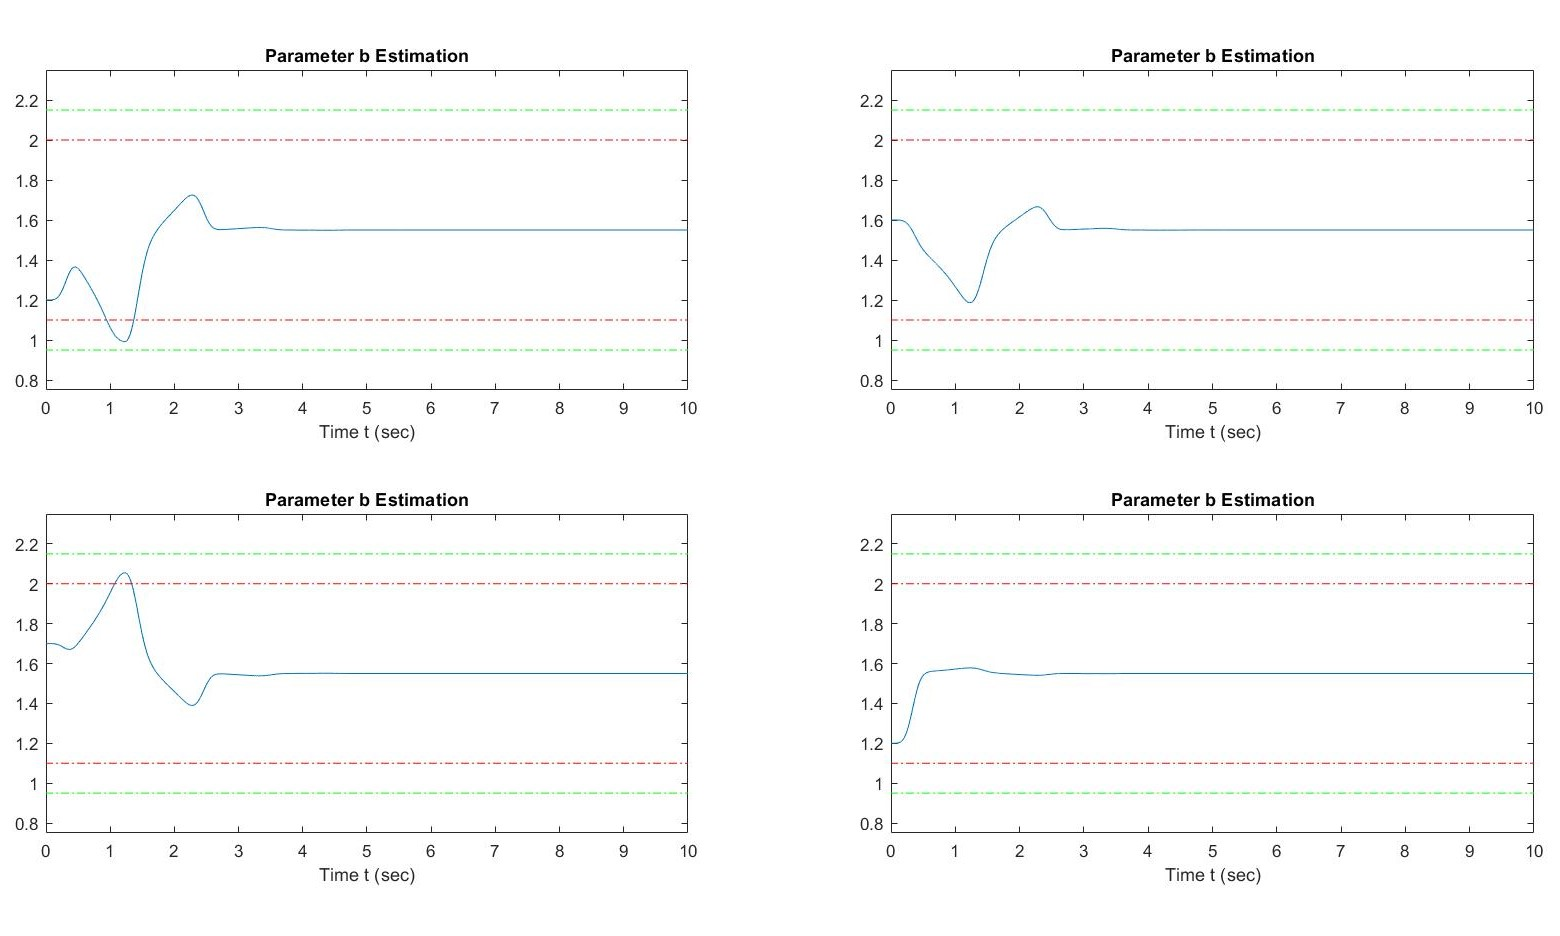
\includegraphics[width=\linewidth]{b_est_b2.jpg}
\centerline{Σχήμα 12:  Χρονική Απόκριση Εκτίμησης $\hat{b} \quad (2)$}
\\ \\
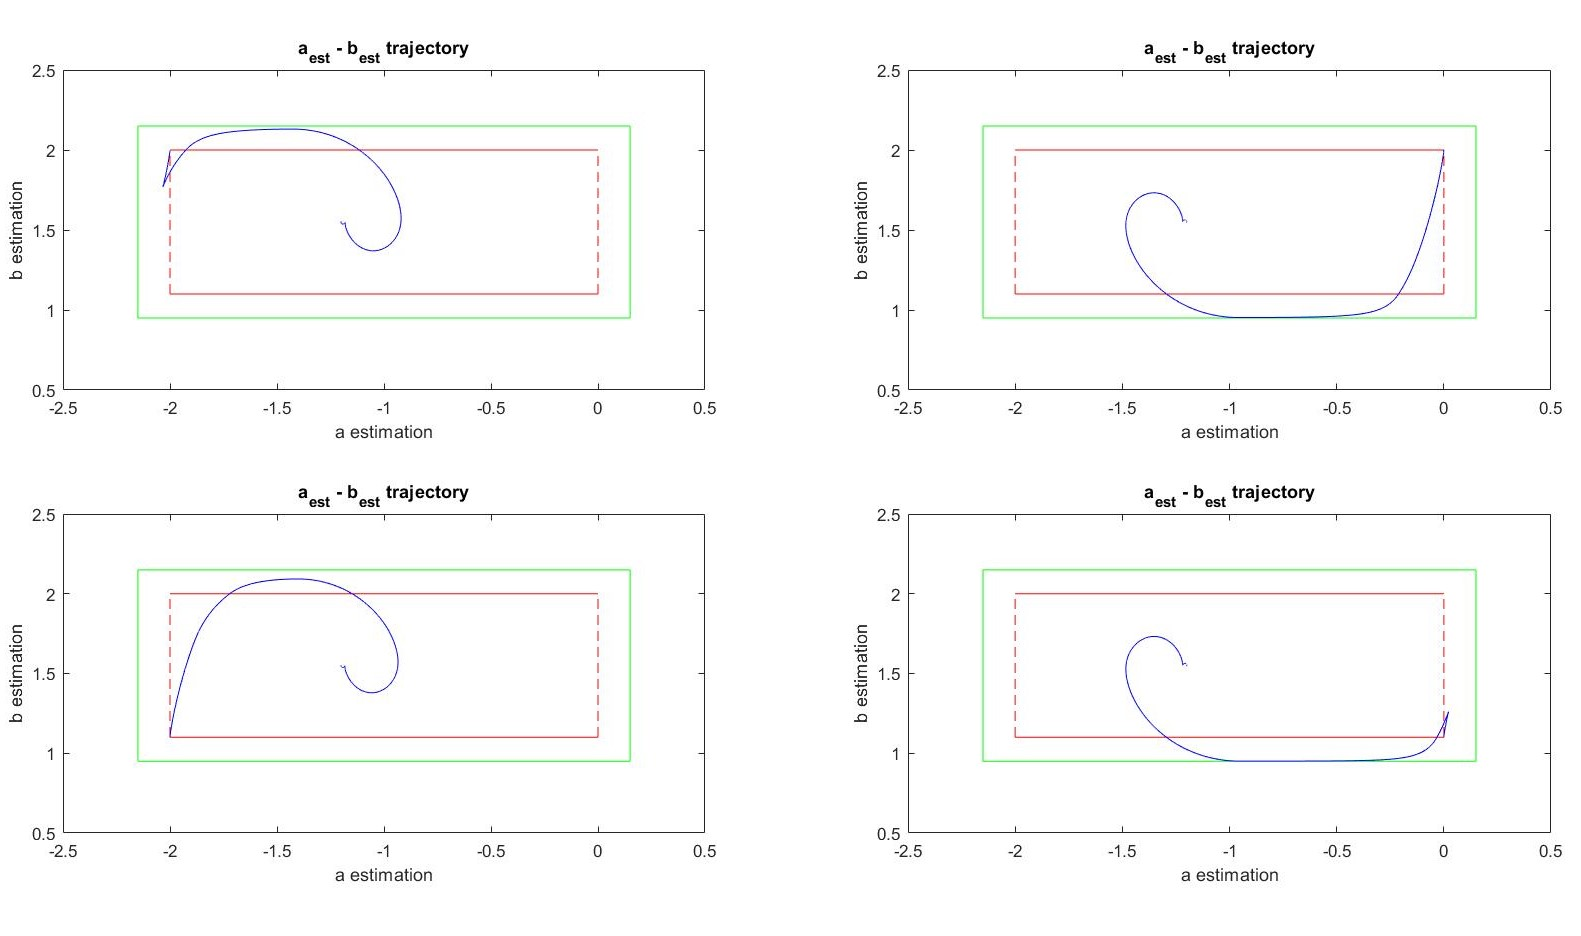
\includegraphics[width=\linewidth]{ab_est_b1.jpg}
\centerline{Σχήμα 13: Τροχιά Εκτιμήσεων στο Επίπεδο $\hat{a} - \hat{b} \quad (1)$}
\\ \\
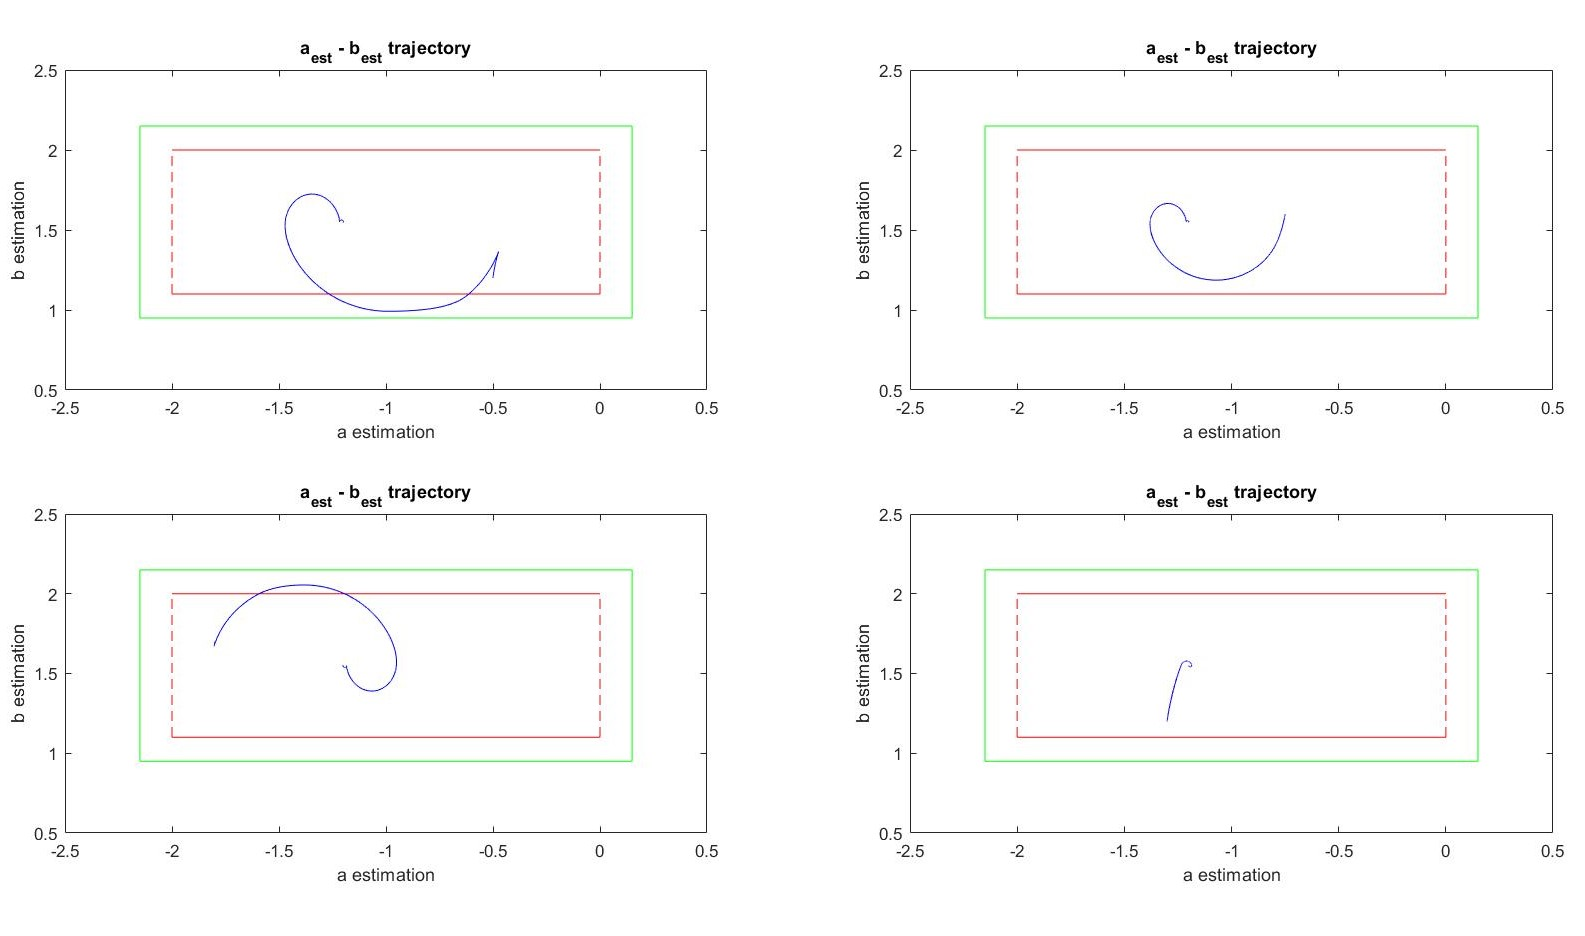
\includegraphics[width=\linewidth]{ab_est_b2.jpg}
\centerline{Σχήμα 14: Τροχιά Εκτιμήσεων στο Επίπεδο $\hat{a} - \hat{b} \quad (2)$}
\\ \\
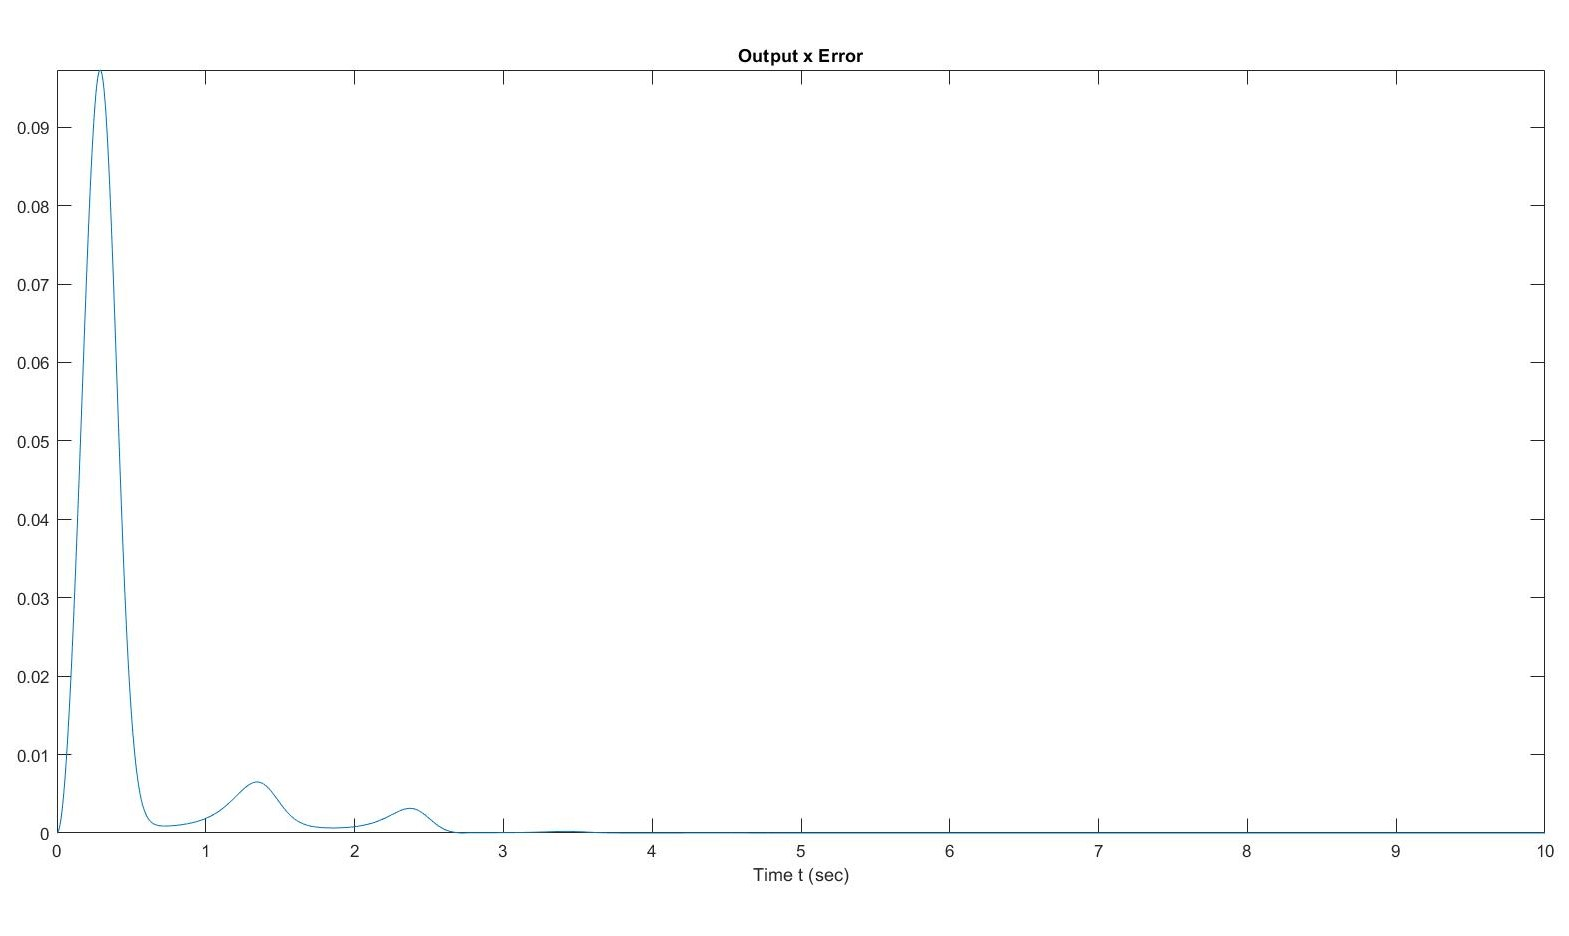
\includegraphics[width=\linewidth]{errorB.jpg}
\centerline{Σχήμα 15:  Χρονική Απόκριση Σφάλματος}
\\ \\
Όπως φαίνεται από τη γραφική παράσταση του Σχήματος 15 η συνάρτηση του σφάλματος είναι πιο ομαλή σε σχέση με τον προηγούμενο αλγόριθμο ενώ παράλληλα συγκλίνει γρηγορότερα στο μηδέν χωρίς έντονες διαταραχές. Αντίστοιχα σφάλματα παρατηρούνται και για τις υπόλοιπες αρχικές τιμές.
\\ \\
Τέλος, γενικότερα από τις γραφικές παραστάσεις των σφαλμάτων και των εκτιμήσεων γίνεται ξεκάθαρο ότι πληρούται η Συνθήκη Επιμένουσας Διέγερσης, αφού υπάρχει σύγκλιση των εκτιμήσεων στις πραγματικές τους τιμές, με τη χρήση και των δύο αλγορίθμων.
\end{document}